\documentclass[11pt,a4paper]{article}

\usepackage[margin=0.85in]{geometry}
\usepackage{amsmath,amssymb}
\usepackage{graphicx}
\usepackage{booktabs}
\usepackage{array}
\usepackage{xcolor}
\usepackage{hyperref}
\usepackage{caption}
\usepackage{enumitem}
\usepackage{float}
\usepackage[T1]{fontenc}
\usepackage[utf8]{inputenc}

\hypersetup{
  colorlinks=true,
  linkcolor=blue!55!black,
  urlcolor=blue!55!black,
  citecolor=blue!55!black,
}

\captionsetup{font=small,labelfont=bf,skip=4pt}

\setlength{\parskip}{4pt}
\setlength{\parindent}{0pt}

% =============================================================================
\title{\vspace{-1.5em}\textbf{Group 6 --- Project Submission Report}\\[4pt]
\large A Comparative Framework for Survival Analysis on the RMS Titanic\\
\normalsize Na\"ive Bayesian vs.\ Decision Tree Classifiers}

\author{%
  Sarin Vadakke Thayyil \quad|\quad Lekshmi S~S \quad|\quad
  Akbar T~E \quad|\quad Suja V \quad|\quad Nikhil Ravi \\[2pt]
  \small eMTech (AI) 2026 Batch \quad|\quad
  Indian Institute of Information Technology, Kottayam \\
  \small DSC 523 --- Data Mining \quad|\quad
  Instructor: Dr.\ Anu Maria Sebastian
}
\date{25 April 2026}

\begin{document}
\maketitle

% =============================================================================
\section*{1. Project Repository}
The complete project --- including the Jupyter notebook, all source scripts, the
Kaggle \texttt{train.csv} dataset, every figure used in the conference paper, and
the compiled paper itself --- is publicly hosted at:

\begin{center}
\href{https://github.com/vtsarin/dsc-523-mini-project}{%
\texttt{https://github.com/vtsarin/dsc-523-mini-project}}
\end{center}

\noindent The conference paper (PDF) and the executable notebook are reproducible
end-to-end from the scripts \texttt{run\_analysis.py},
\texttt{build\_notebook.py}, and \texttt{make\_flowchart.py}; all stochastic
components use \texttt{random\_state = 42}.

% =============================================================================
\section*{2. Member Contribution Table}

\renewcommand{\arraystretch}{1.35}
\begin{table}[H]
\centering
\caption{Group 6 --- Member contributions.}
\small
\begin{tabular}{@{}p{0.20\textwidth}p{0.30\textwidth}p{0.42\textwidth}@{}}
\toprule
\textbf{Member's Name} & \textbf{Sections Written} & \textbf{Tasks Undertaken} \\
\midrule
Sarin Vadakke Thayyil
& \S1 Introduction; \S4 Methodology; \S6 Implications and Applications;
  \S7 Conclusion (final consolidation)
& Project management and team coordination; defined the 80/20 stratified
  evaluation protocol; designed the comparative experimental framework;
  authored and assembled the final manuscript; managed deliverables and
  GitHub repository.
\\
\addlinespace
Lekshmi S~S
& \S2 Literature Review (all five subsections including Research Gap and
  Motivation)
& Comparative analysis of Gini vs.\ entropy impurity measures; literature
  survey of NB, DT, LR, RF on the Titanic benchmark; identified the research
  gap; framed the theoretical foundations.
\\
\addlinespace
Akbar T~E
& Figure captions and visual narrative across \S3, \S4, \S5
& Produced all 11 figures (KDD flowchart, EDA panels, age-fare distribution,
  correlation heatmap, confusion matrices, ROC curves, feature importances,
  decision-tree visualisation); designed the consistent colour palette and
  matplotlib styling; built \texttt{make\_flowchart.py}.
\\
\addlinespace
Suja V
& \S3 Dataset Description; \S4.1 Data Profiling; \S4.2 Missing-Value
  Treatment; \S4.3 Feature Engineering; \S4.4 Encoding
& Designed the group-wise (\texttt{Pclass}$\times$\texttt{Sex}) median
  imputation rule for \texttt{Age}; mined the \texttt{Cabin} field for the
  \texttt{Deck} feature; engineered \texttt{Title}, \texttt{FamilySize},
  \texttt{IsAlone}, \texttt{AgeBin} and \texttt{FareBin}; built the encoding
  pipeline and verified zero residual missingness.
\\
\addlinespace
Nikhil Ravi
& \S5 Results and Discussion (including \S5.2 Model Performance, \S5.3
  Statistical Significance, \S5.4 Discussion)
& Implemented and ran all four classifiers; computed 10-fold stratified CV
  scores; verified every confusion matrix; ran the McNemar exact paired
  test ($p = 8.22\times 10^{-6}$); produced \texttt{results.json};
  reviewed manuscript for compliance with course guidelines.
\\
\bottomrule
\end{tabular}
\end{table}

% =============================================================================
\section*{3. Visualisations}

\begin{figure}[H]
\centering
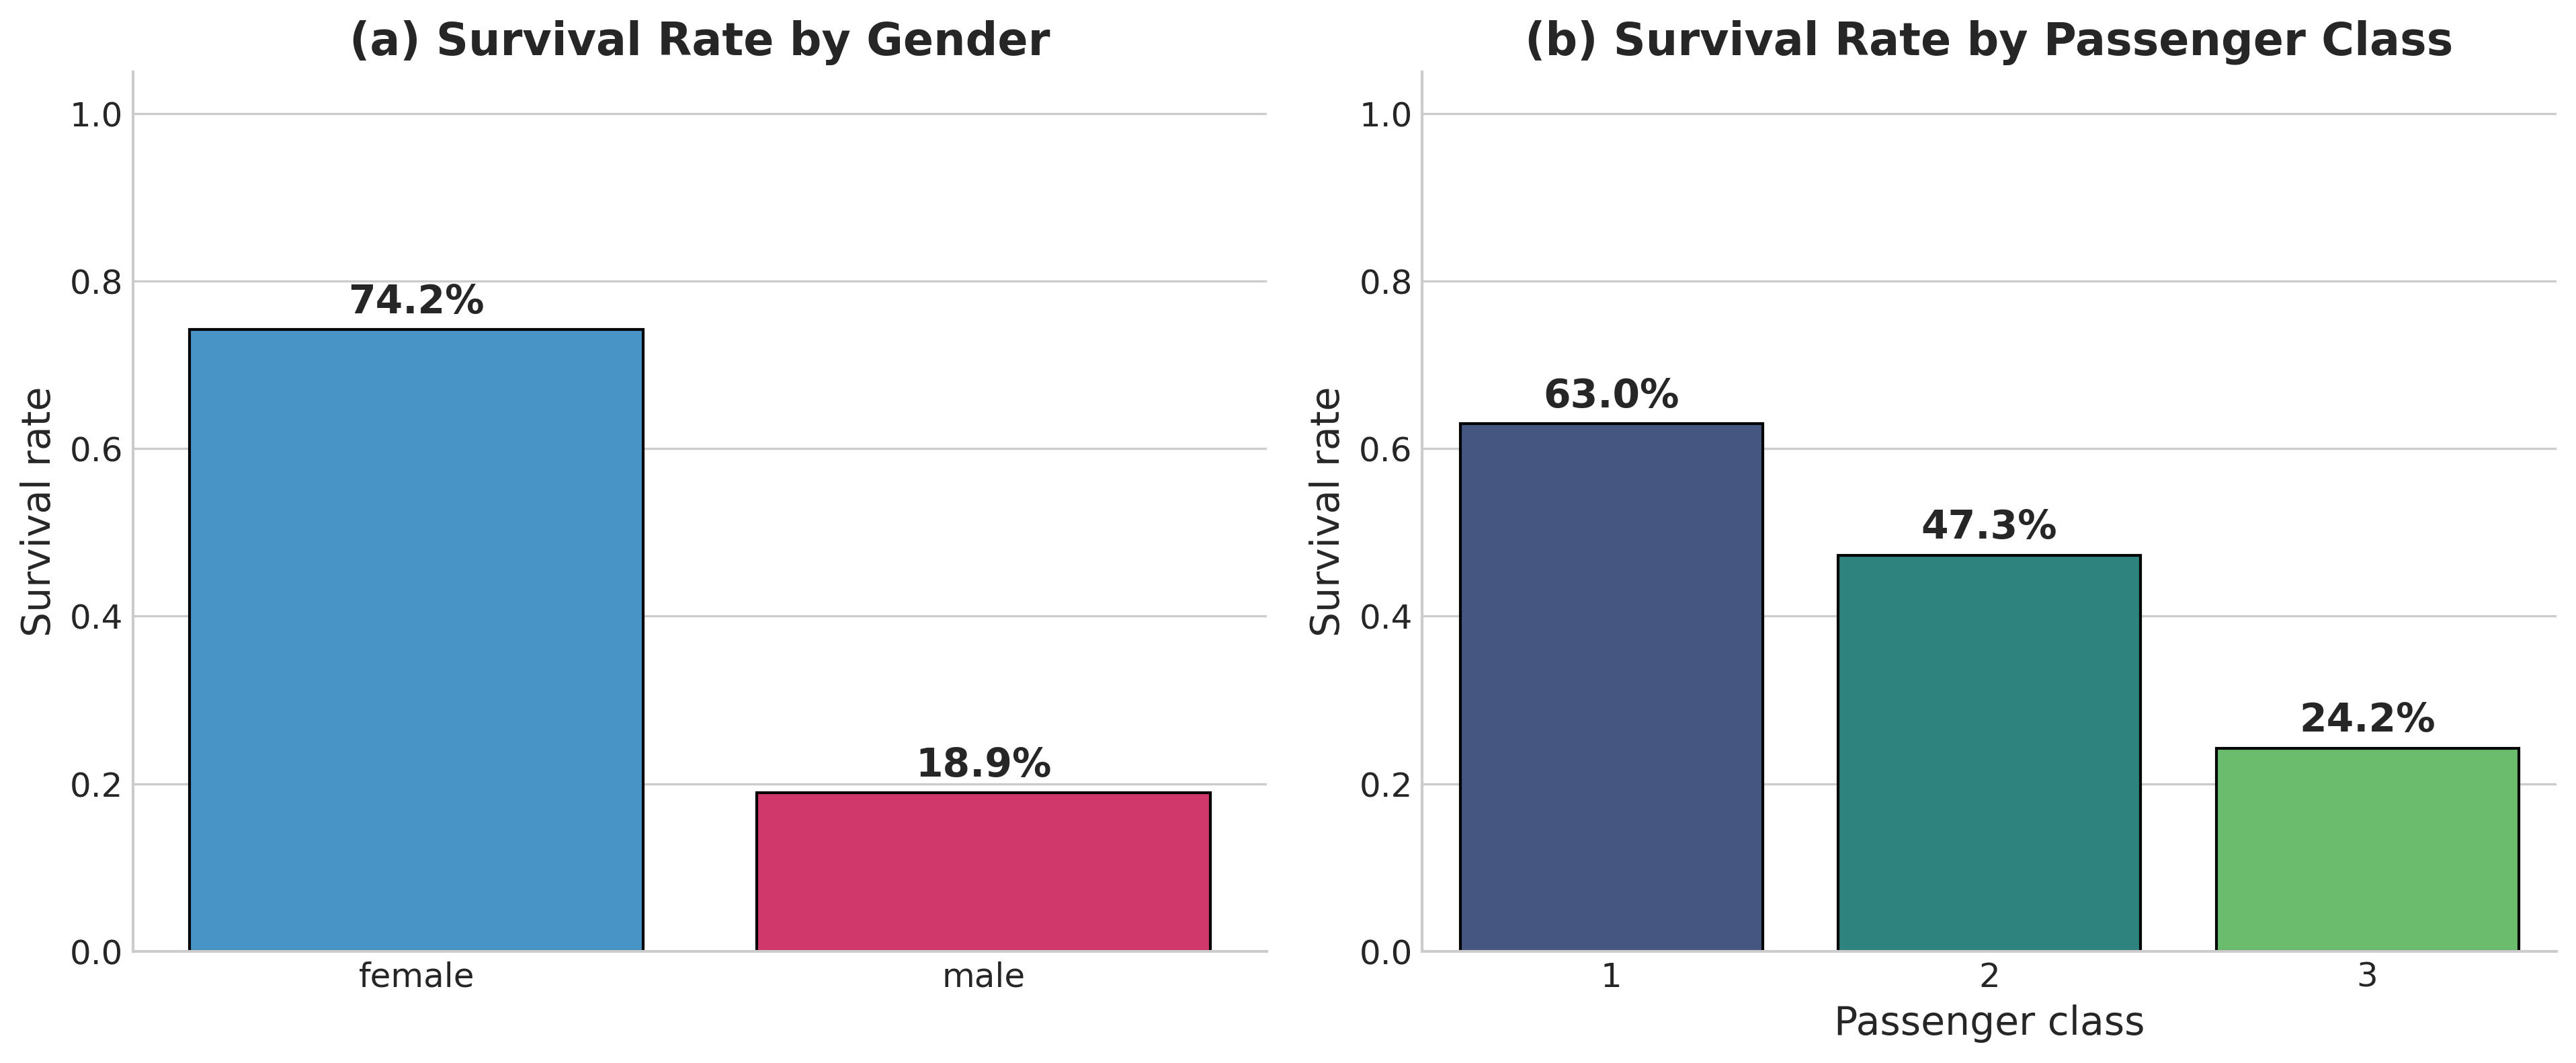
\includegraphics[width=0.96\textwidth]{figures/survival_gender_class_panel.png}
\caption{Univariate survival rates by the two strongest predictors. Female
passengers survived at 74.2\% versus 18.9\% for males; survival declines
monotonically with passenger class.}
\end{figure}

\begin{figure}[H]
\centering
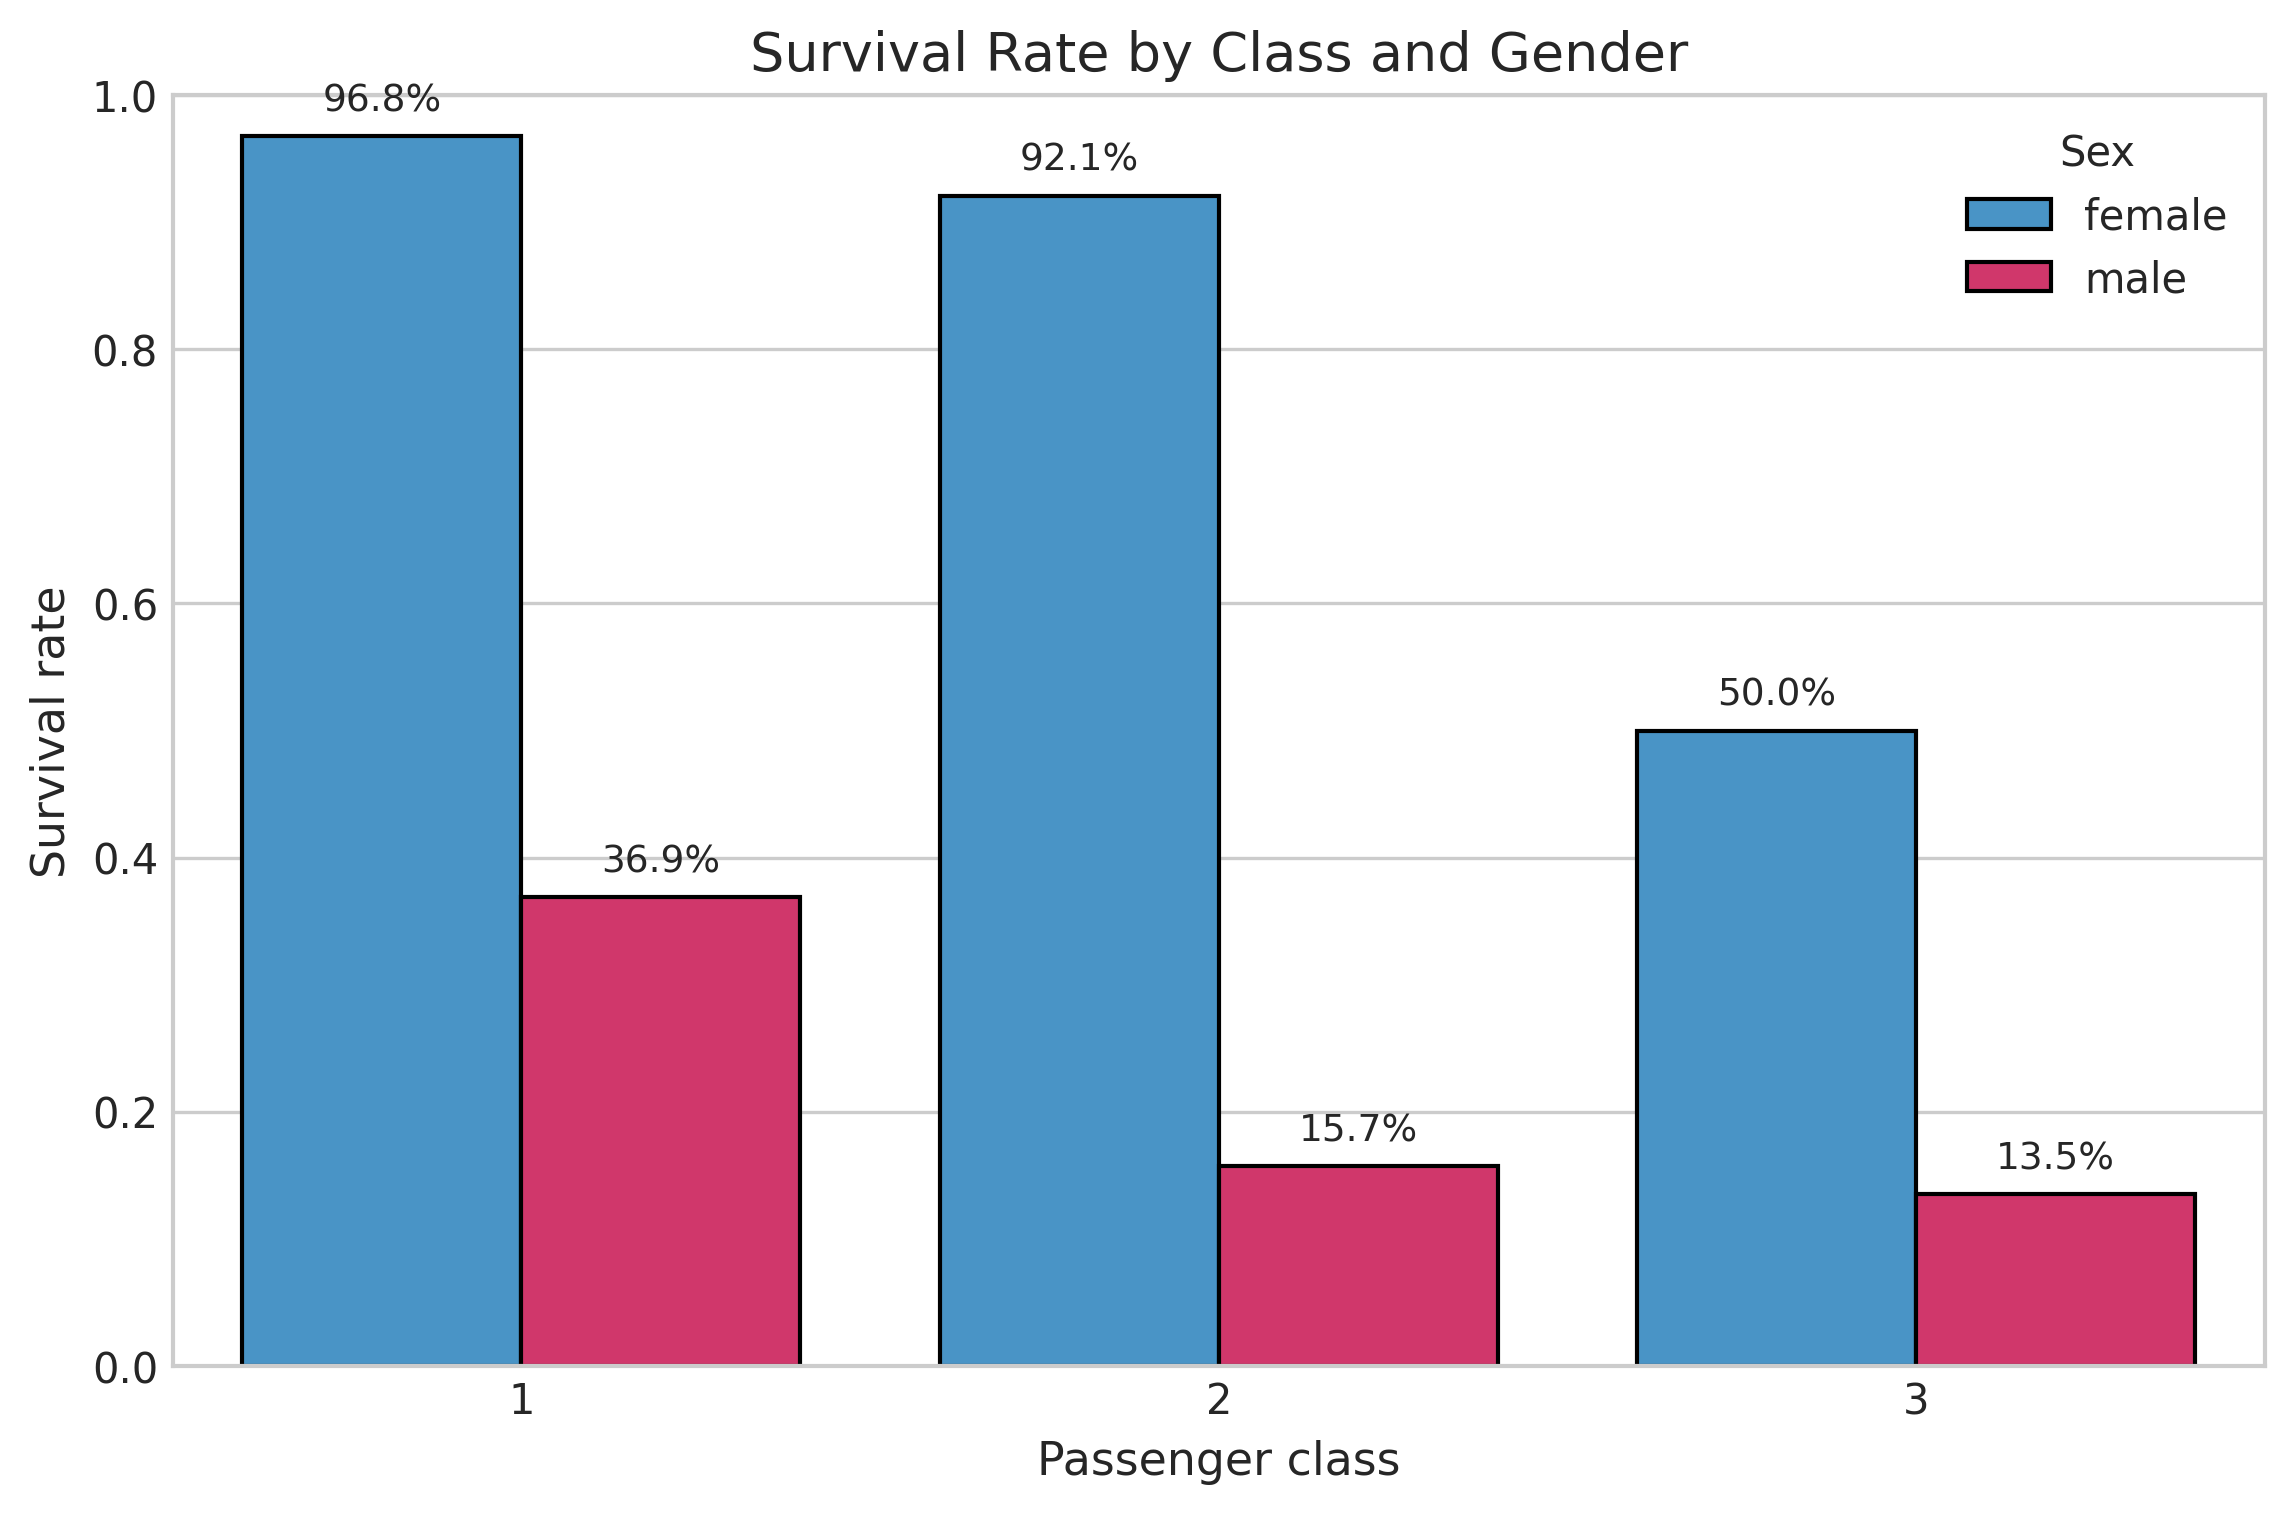
\includegraphics[width=0.65\textwidth]{figures/survival_by_class_gender.png}
\caption{Joint effect of class and gender. First-class women survived at 96.8\%;
third-class men survived at only 13.5\%.}
\end{figure}

\begin{figure}[H]
\centering
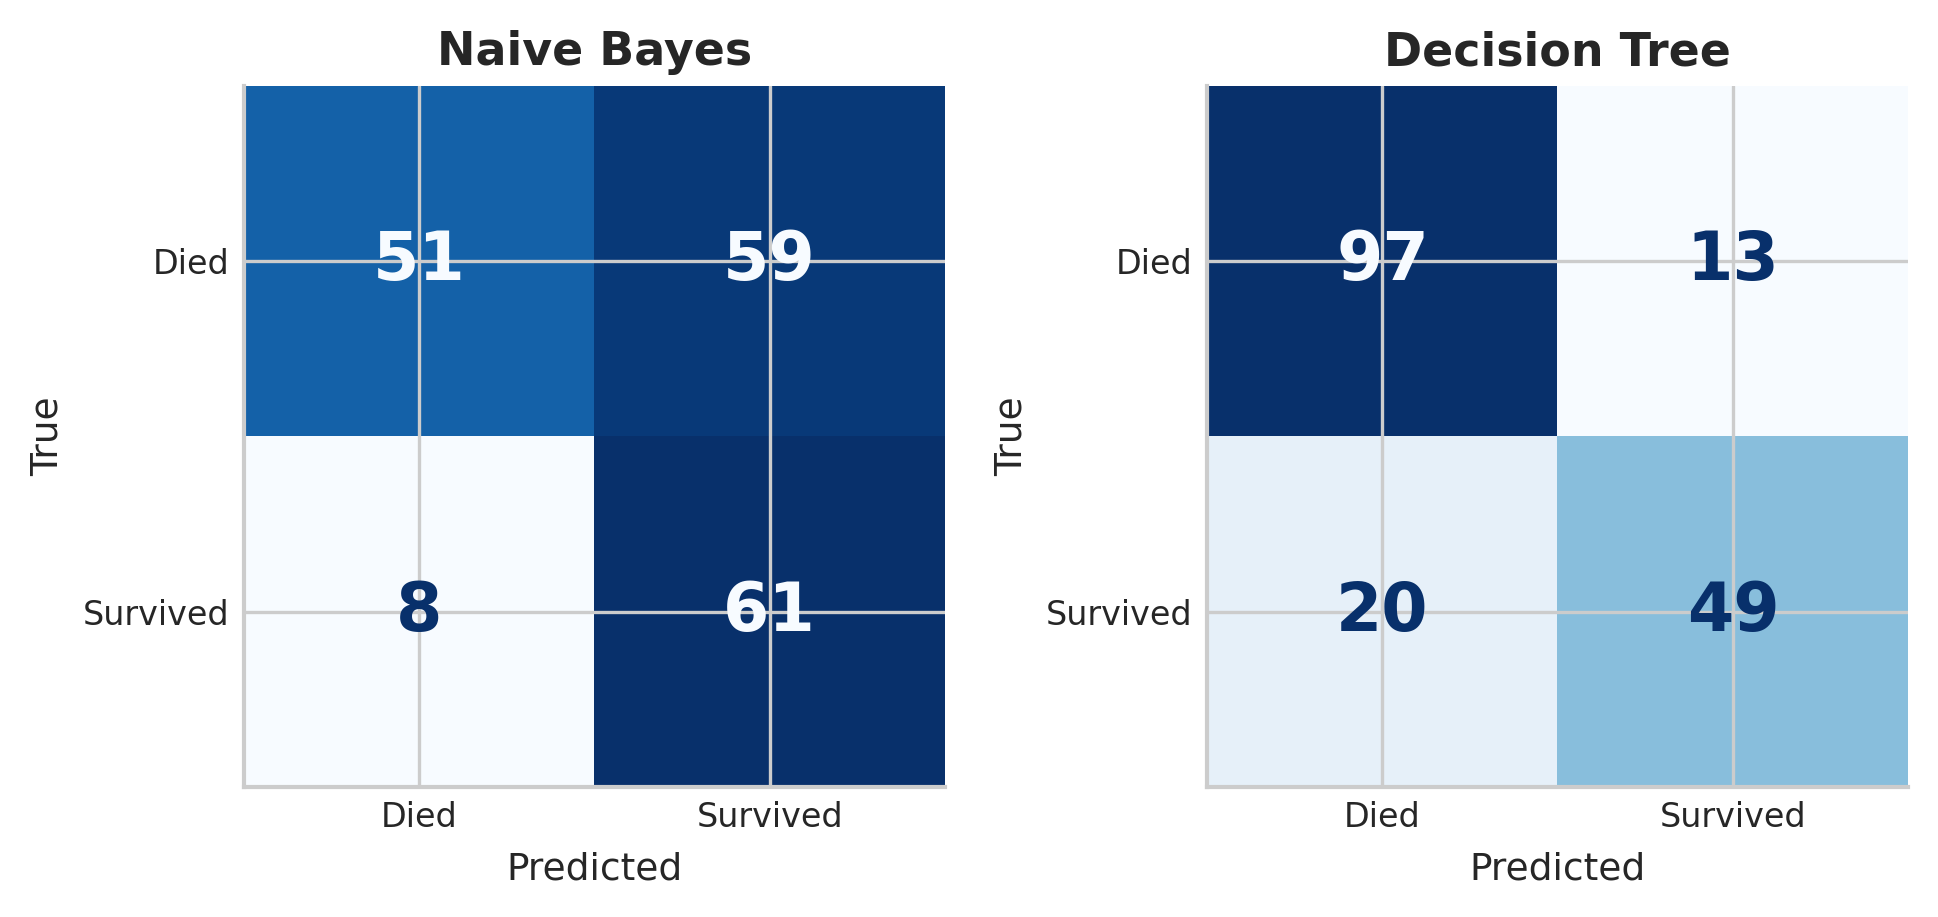
\includegraphics[width=0.85\textwidth]{figures/confusion_matrices_panel.png}
\caption{Confusion matrices on the held-out test set. Na\"ive Bayes over-predicts
the positive class (59 false positives); the Decision Tree is materially better
balanced (only 13 false positives).}
\end{figure}

\begin{figure}[H]
\centering
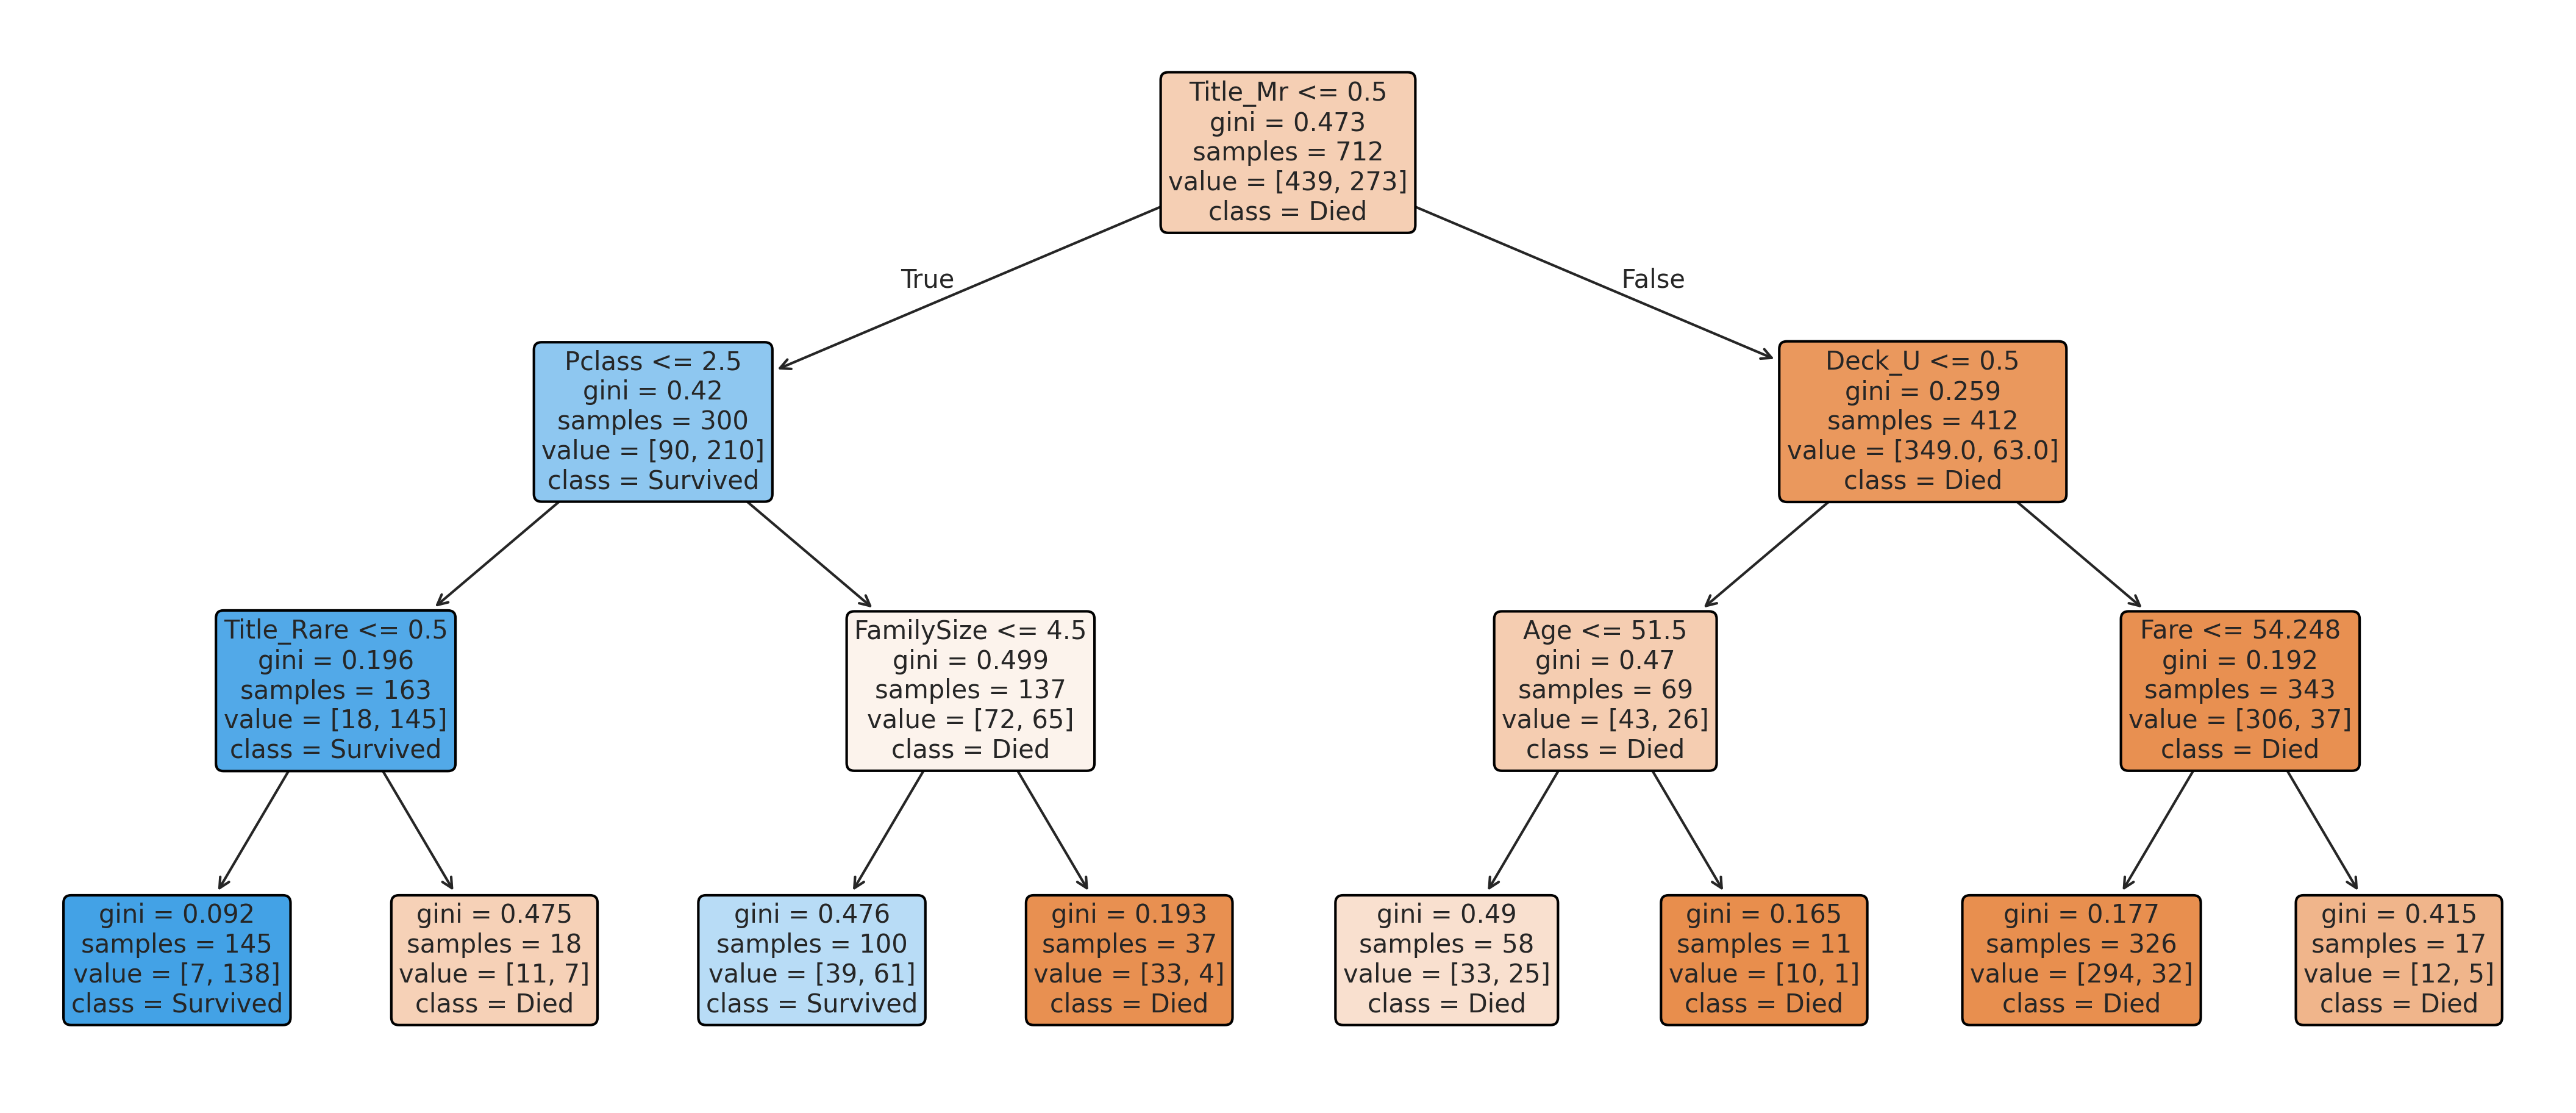
\includegraphics[width=0.96\textwidth]{figures/decision_tree_viz.png}
\caption{Fitted Decision Tree (\texttt{max\_depth}=3 shown for readability;
deployed model uses depth~4). The root split on \texttt{Title\_Mr} captures the
bulk of the gender / honorific signal in a single question.}
\end{figure}

\begin{figure}[H]
\centering
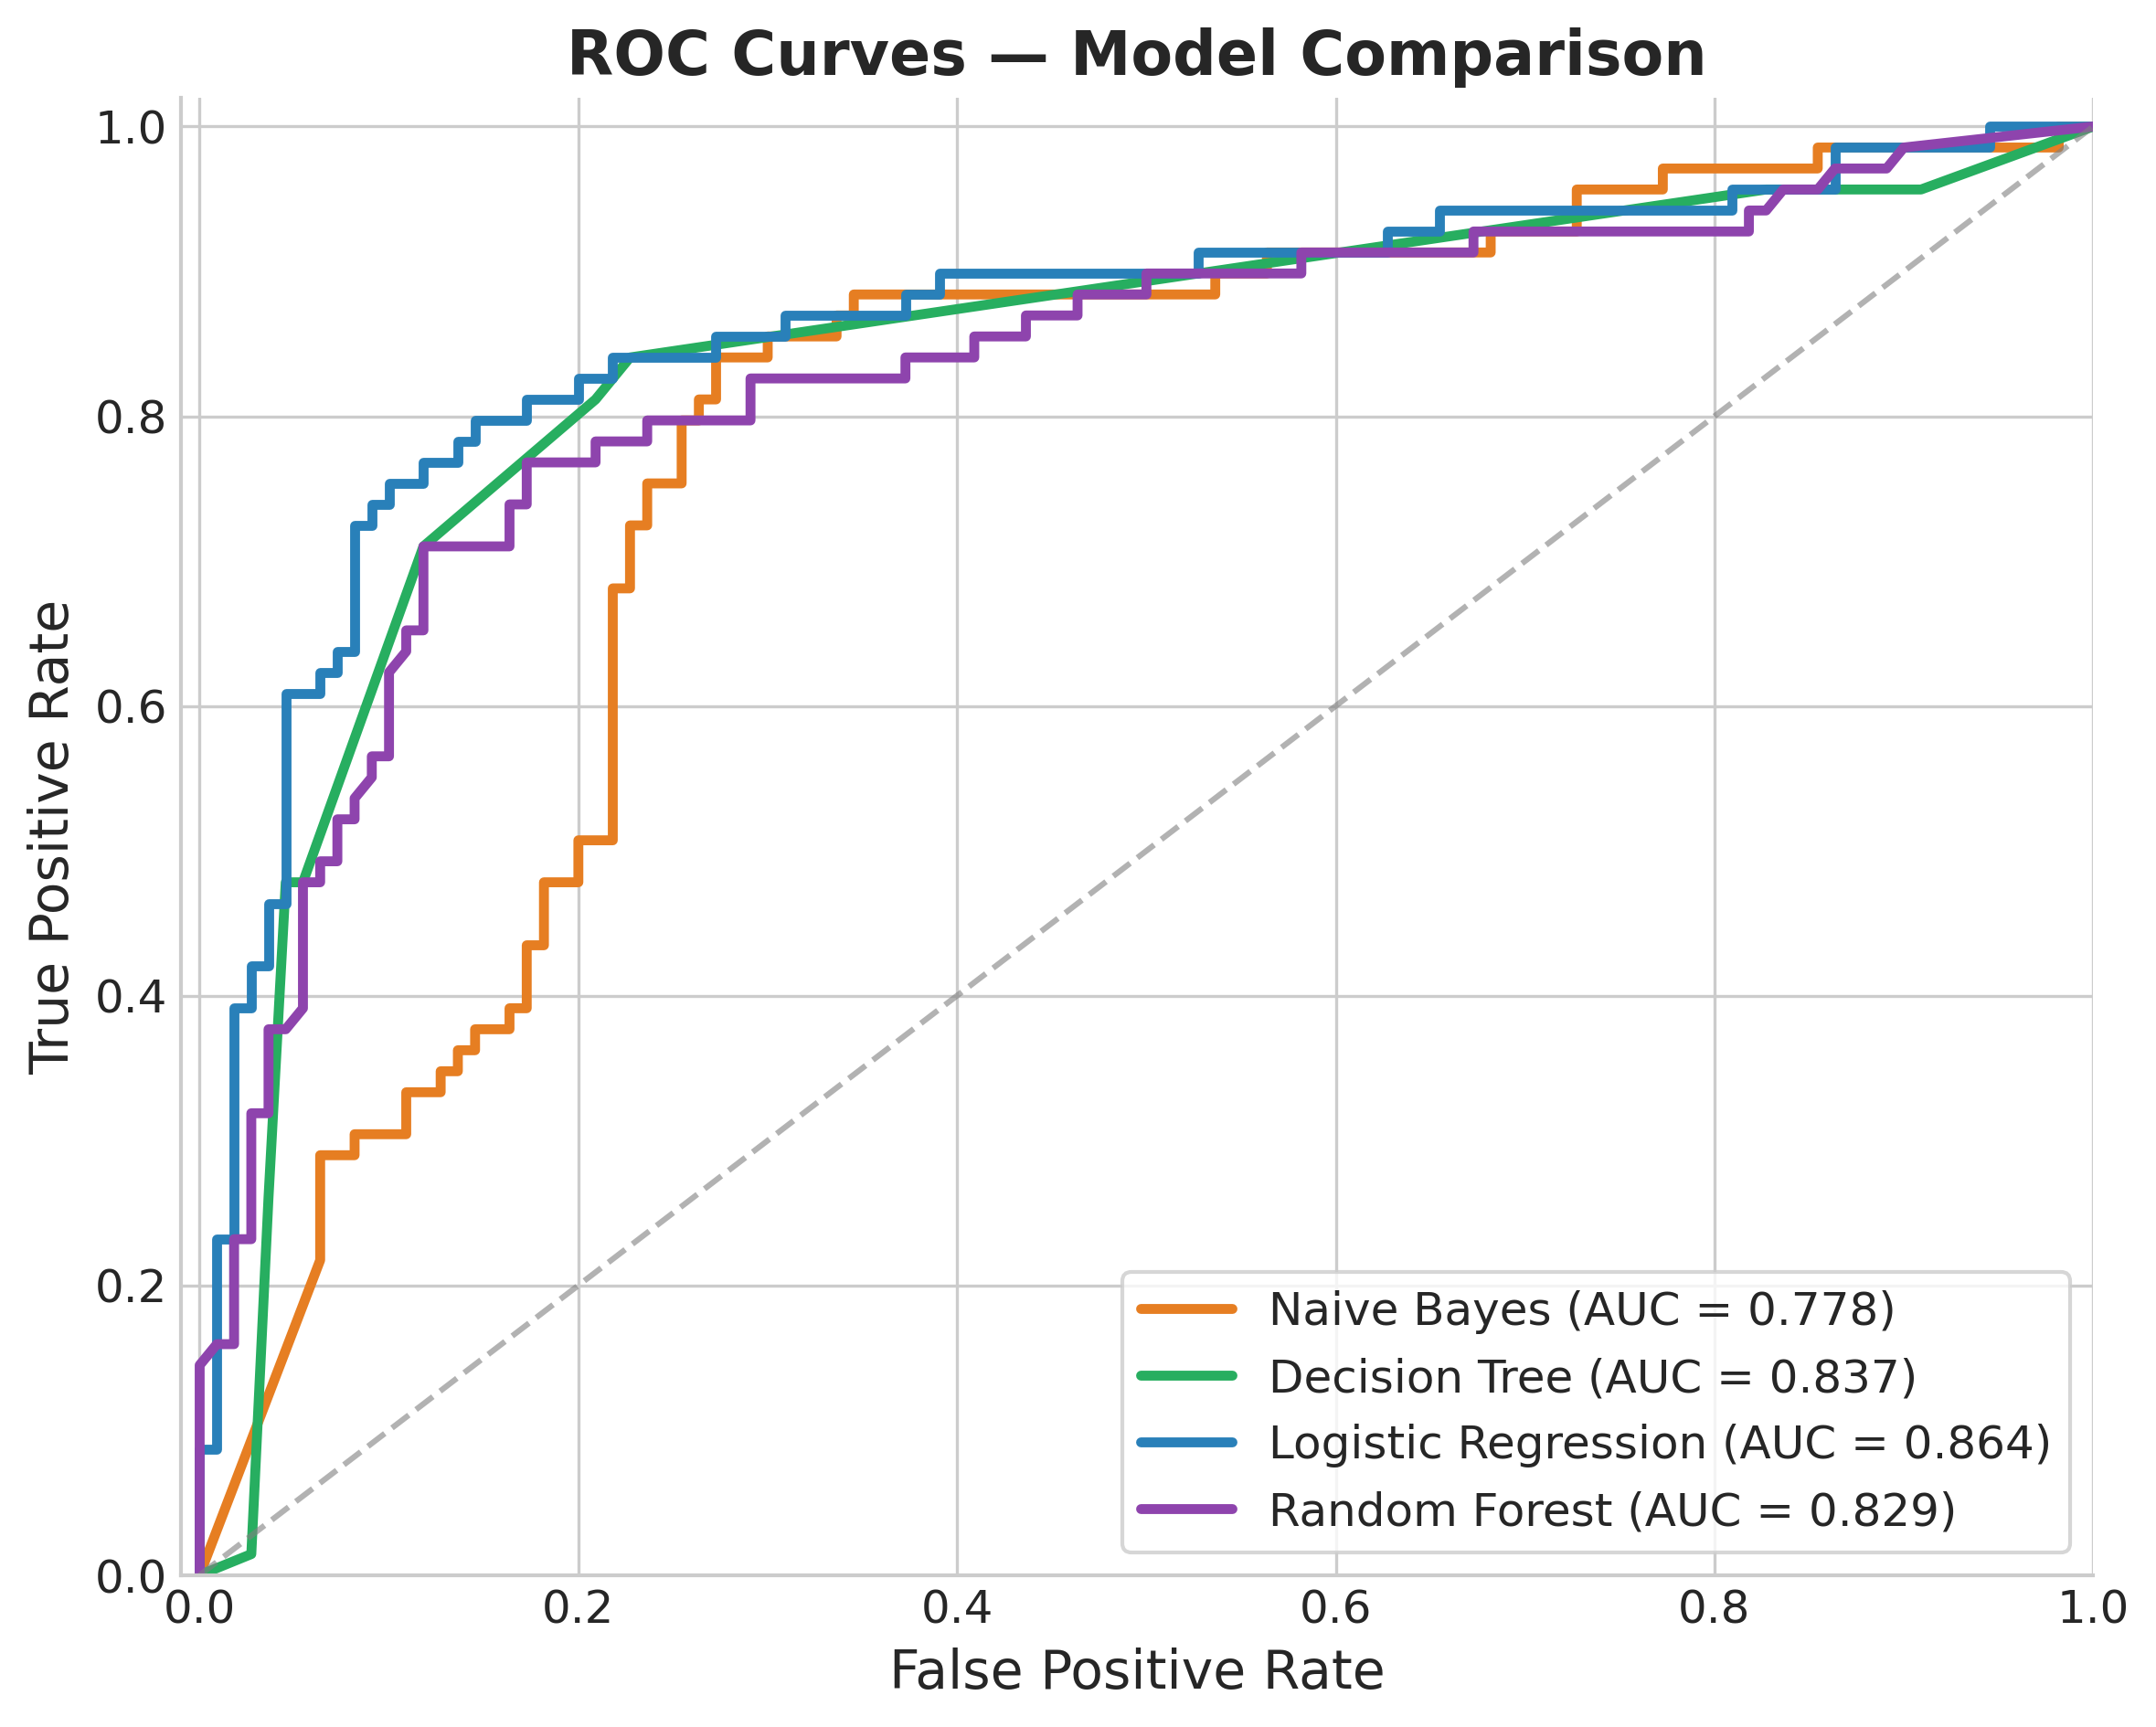
\includegraphics[width=0.7\textwidth]{figures/roc_curves.png}
\caption{ROC curves for all four classifiers. Logistic Regression dominates
slightly across most thresholds (AUC $= 0.864$); Na\"ive Bayes trails uniformly.}
\end{figure}

% =============================================================================
\section*{4. Most Important Findings}

\begin{enumerate}[leftmargin=1.3em,itemsep=4pt]

\item \textbf{The Decision Tree decisively outperforms Na\"ive Bayes by
\textasciitilde 19 percentage points.}
On the held-out test set ($n_\text{test}=179$), the Decision Tree achieves
$81.56\%$ accuracy (AUC $= 0.838$) while Gaussian Na\"ive Bayes reaches only
$62.57\%$ (AUC $= 0.778$). McNemar's exact paired test gives
$p = 8.22\times 10^{-6}$, rejecting the null of equal error rates at any
conventional level --- the gap is not a sampling artefact.

\item \textbf{Logistic Regression is the strongest single model overall.}
After feature engineering, the decision boundary is close to linear: Logistic
Regression attains $83.24\%$ test accuracy and AUC $= 0.864$. Random Forest
($81.01\%$) does not outperform the single Decision Tree, suggesting the
engineered feature set already captures the important interactions.

\item \textbf{Gender dominates; class modulates.}
Female passengers survived at $74.2\%$ versus $18.9\%$ for males
($\chi^2 = 260.7$, $p = 1.2\times 10^{-58}$). Survival declines monotonically
with class: 1st (63.0\%), 2nd (47.3\%), 3rd (24.2\%). The interaction is
striking --- 1st-class women survived at $96.8\%$ (91 of 94) while 3rd-class
men survived at only $13.5\%$ (47 of 347).

\item \textbf{Family size has a non-monotonic effect.}
Survival peaks at family sizes of 2--4 (55--72\%) and collapses for solo
passengers (30.4\%) and very large families of $\ge 5$ (16\%) --- a pattern
neither \texttt{SibSp} nor \texttt{Parch} captures alone, justifying the
engineered \texttt{FamilySize} feature.

\item \textbf{NB fails because multicollinearity violates its independence
assumption.}
After feature engineering, several feature pairs are strongly correlated by
construction: $r(\texttt{SibSp},\texttt{FamilySize}) = +0.89$,
$r(\texttt{Sex\_female},\texttt{Title\_Mr}) = -0.87$,
$r(\texttt{Parch},\texttt{FamilySize}) = +0.78$. These violate the
class-conditional independence assumption directly, compounding the per-feature
evidence terms and distorting the NB posterior --- the textbook failure mode of
Gaussian NB on engineered tabular data.

\end{enumerate}

\end{document}
